\documentclass[aspectratio=169,11pt]{beamer}

\usepackage[utf8]{inputenc}
\usepackage[T1]{fontenc}
\usepackage[english]{babel}
\usepackage{amsmath,amssymb,mathtools}
\usepackage{booktabs,array}
\usepackage{tikz}
\usetikzlibrary{arrows.meta,positioning}

\definecolor{navy}{HTML}{17324D}
\definecolor{blue}{HTML}{247BA0}
\definecolor{teal}{HTML}{2A9D8F}
\definecolor{gold}{HTML}{E9A23B}
\definecolor{red}{HTML}{C14953}
\definecolor{pale}{HTML}{F2F6F8}
\definecolor{ink}{HTML}{17212B}

\usetheme{default}
\usefonttheme{professionalfonts}
\setbeamertemplate{navigation symbols}{}
\setbeamertemplate{itemize item}{\color{teal}$\blacktriangleright$}
\setbeamertemplate{itemize subitem}{\color{blue}$\bullet$}
\setbeamercolor{normal text}{fg=ink,bg=white}
\setbeamercolor{structure}{fg=navy}
\setbeamercolor{frametitle}{fg=white,bg=navy}
\setbeamerfont{frametitle}{series=\bfseries,size=\large}
\setbeamercolor{block title}{fg=white,bg=blue}
\setbeamercolor{block body}{fg=ink,bg=pale}
\setbeamercolor{alerted text}{fg=red}
\setbeamercolor{leanbox}{fg=ink,bg=pale}
\setbeamertemplate{frametitle}{%
  \nointerlineskip
  \begin{beamercolorbox}[wd=\paperwidth,ht=2.9ex,dp=1.1ex,leftskip=.55cm]{frametitle}
    \insertframetitle
  \end{beamercolorbox}}
\setbeamertemplate{footline}{%
  \leavevmode%
  \hbox{%
    \begin{beamercolorbox}[wd=.78\paperwidth,ht=2.5ex,dp=1ex,leftskip=.45cm]{author in head/foot}%
      \color{navy}\scriptsize Ide \& Talam\`as (2025) \textperiodcentered{} arXiv v11
    \end{beamercolorbox}%
    \begin{beamercolorbox}[wd=.22\paperwidth,ht=2.5ex,dp=1ex,rightskip=.45cm plus 1fil]{date in head/foot}%
      \color{navy}\scriptsize\hfill\insertframenumber/\inserttotalframenumber
    \end{beamercolorbox}}}

\newcommand{\zAI}{z_{\mathrm{AI}}}
\newcommand{\zbAI}{\bar z_{\mathrm{AI}}}
\newcommand{\wA}{w^{A}}
\newcommand{\wN}{w^{N}}
\newcommand{\YA}{Y^{A}}
\newcommand{\YN}{Y^{N}}
\newcommand{\key}[1]{\textcolor{teal}{\textbf{#1}}}

\title{Artificial Intelligence in the Knowledge Economy}
\subtitle{Capability, autonomy, organization, and the distribution of gains}
\author{Carlos G\'omez Puican\\[1mm]\small Paper by Enrique Ide \& Eduard Talam\`as}
\institute{Repository 5}
\date{arXiv v11 \textperiodcentered{} February 25, 2025 \textperiodcentered{} 35 pages}

\begin{document}

% Title slide (not counted among the 15 substantive slides)
\begin{frame}[plain]
  \titlepage
  \vspace{-1.2em}
  \begin{center}
    \small
    \href{https://github.com/carlosgomezp28/ai-05-ide}%
      {\texttt{https://github.com/carlosgomezp28/ai-05-ide}}
  \end{center}
\end{frame}

% 1
\begin{frame}{1. Research question and contribution}
  \begin{block}{Question}
    How does scalable AI that can acquire tacit knowledge reorganize knowledge work---and who gains when AI can act rather than merely advise?
  \end{block}

  \begin{columns}[T,onlytextwidth]
    \column{.49\textwidth}
      \key{Organizational margin}
      \begin{itemize}\small
        \item Humans sort into routine production and exceptional problem solving.
        \item AI changes occupations, matching, spans of control, and wages in equilibrium.
      \end{itemize}
    \column{.49\textwidth}
      \key{Two technological dimensions}
      \begin{itemize}\small
        \item Capability: how difficult a problem AI can solve.
        \item Autonomy: whether AI can pursue work independently or only assist.
      \end{itemize}
  \end{columns}

  \medskip
  \centering
  \textbf{Central tradeoff:} autonomous AI raises output more, but directs relatively more gains toward the top.
\end{frame}

% 2
\begin{frame}{2. Before AI: a knowledge hierarchy}
  Humans have observable knowledge $z\in[0,1]$, with CDF $G$ and a continuous, strictly positive density.

  \medskip
  \begin{center}
  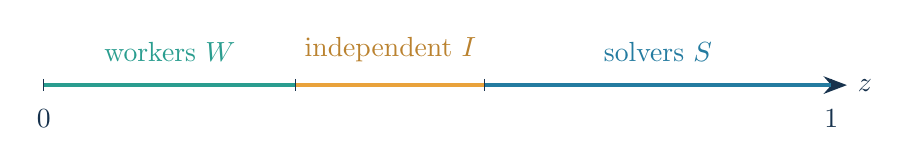
\begin{tikzpicture}[x=1cm,y=1cm,>=Stealth]
    \draw[very thick,->,navy] (0,0)--(10.2,0) node[right] {$z$};
    \draw[very thick,teal] (0,0)--(3.2,0);
    \draw[very thick,gold] (3.2,0)--(5.6,0);
    \draw[very thick,blue] (5.6,0)--(10,0);
    \foreach \x/\lab in {0/0,3.2/{},5.6/{},10/1}
      \draw[navy] (\x,.08)--(\x,-.08) node[below=3pt] {\lab};
    \node[above=5pt,teal] at (1.6,0) {workers $W$};
    \node[above=5pt,gold!80!black] at (4.4,0) {independent $I$};
    \node[above=5pt,blue] at (7.8,0) {solvers $S$};
  \end{tikzpicture}
  \end{center}

  \begin{itemize}\small
    \item An independent producer spends one unit of time on one opportunity.
    \item Workers attempt routine cases; solvers handle the exceptions workers cannot solve.
    \item Knowledge is tacit: the worker must ask before learning whether the solver knows the answer.
    \item Equilibrium exhibits \key{management by exception}: $W\preceq I\preceq S$, with positive assortative matching.
  \end{itemize}
\end{frame}

% 3
\begin{frame}{3. The economic problem and team size}
  A problem has difficulty $x\sim U[0,1]$. Knowledge $z$ therefore has a direct interpretation:
  \[
    \Pr(\text{solve independently}\mid z)=\Pr(x\le z)=z.
  \]

  A worker fails with probability $1-z$. Each request consumes $h\in(0,1)$ units of solver time, so full use of one solver requires
  \[
    h\,n(z)(1-z)=1
    \qquad\Longrightarrow\qquad
    \boxed{n(z)=\frac{1}{h(1-z)}}.
  \]

  Firms choose the organization that maximizes expected output net of wages and compute rent. For a human solver $s$ and human workers $z$,
  \[
    \Pi^{nA}_2(s,z)=n(z)\,[s-w(z)]-w(s),\qquad z\le s.
  \]

  \smallskip
  \centering
  Competition imposes non-positive feasible profits, zero profit for used configurations, and market clearing.
\end{frame}

% 4
\begin{frame}{4. AI technology: capability is not autonomy}
  One unit of compute creates an AI agent. Keep the two dimensions separate:

  \medskip
  \begin{tabular}{>{\bfseries}p{.19\textwidth}p{.35\textwidth}p{.38\textwidth}}
    \toprule
      & Capability $\zAI$ & Autonomy \\
    \midrule
    Meaning
      & Knowledge cutoff: fraction of difficulties AI can solve
      & Feasible roles: whether AI may pursue production independently \\[1mm]
    Values
      & $\zAI\in[0,1)$
      & Two paper benchmarks: autonomous or non-autonomous \\[1mm]
    Labels
      & Basic if $\zAI\in\operatorname{int}W$; advanced if $\zAI\in\operatorname{int}S$
      & Autonomous $=$ co-worker and co-pilot; non-autonomous $=$ co-pilot only \\
    \bottomrule
  \end{tabular}

  \medskip
  \begin{block}{Controlled comparison}
    Proposition 6 holds $\zAI$ fixed and changes autonomy. Proposition 5 varies $\zAI$ within the autonomous regime.
  \end{block}
\end{frame}

% 5
\begin{frame}{5. Post-AI firms and equilibrium intuition}
  \small
  \renewcommand{\arraystretch}{1.18}
  \begin{tabular}{p{.28\textwidth}p{.33\textwidth}p{.31\textwidth}}
    \toprule
    Configuration & Profit & Economic role \\
    \midrule
    Independent human & $z-w(z)$ & Human pursues one opportunity \\
    Independent AI & $\zAI-r$ & AI pursues an opportunity \\
    Human team & $n(z)[s-w(z)]-w(s)$ & Human workers, human solver \\
    AI solver (top automated) & $n(z)[\zAI-w(z)]-r$ & Human workers, AI co-pilot \\
    AI workers (bottom automated) & $n(\zAI)[s-r]-w(s)$ & AI co-workers, human solver \\
    \bottomrule
  \end{tabular}

  \medskip
  \begin{itemize}\small
    \item Autonomous AI can enter all three AI roles. Abundant compute guarantees some independent AI production, which pins down $r^*=\zAI$.
    \item Non-autonomous AI cannot be an independent producer or worker; only the top-automated configuration remains available.
    \item Scalability makes AI a large homogeneous supply of knowledge, so its effect is not the same as adding heterogeneous humans.
  \end{itemize}
\end{frame}

% 6
\begin{frame}{6. Propositions 1--4: setup for distributional results}
  \begin{columns}[T,onlytextwidth]
    \column{.49\textwidth}
      \begin{block}{Propositions 1--2: equilibrium}
      \small
      \begin{itemize}
        \item Pre-AI equilibrium: unique, efficient, $W\preceq I\preceq S$, positive assortative matching.
        \item Under $h<h_0$, $I=\varnothing$.
        \item Autonomous-AI equilibrium: unique and efficient, with
          \[
          W^*\preceq\{\zAI\}\preceq S^*.
          \]
        \item AI always does some independent production and $r^*=\zAI$.
      \end{itemize}
      \end{block}
    \column{.49\textwidth}
      \begin{block}{Propositions 3--4: reorganization}
      \small
      \begin{itemize}
        \item Basic AI: $W^*\subset W$, $S\subset S^*$; marginal humans move toward solving.
        \item Advanced AI: $W\subset W^*$, $S^*\subset S$; movement reverses.
        \item Continuing workers' productivity and continuing solvers' spans depend on how AI changes their matches.
      \end{itemize}
      \end{block}
  \end{columns}
  \centering
  \key{Occupational displacement changes both productivity and the division of team output.}
\end{frame}

% 7
\begin{frame}{7. Proposition 5: who wins with autonomous AI?}
  Let $w$ be the pre-AI wage and $\wA$ the autonomous-AI wage. Define
  \[
    B=\{z\in[0,\zAI]:\wA(z)>w(z)\},\qquad
    T=\{z\in[\zAI,1]:\wA(z)>w(z)\}.
  \]

  \begin{block}{Proposition 5}
    Under $h<h_0$, competitive pre/post equilibria, $\zAI\in[0,1)$, and compute abundance uniformly over admissible capabilities, there is
    \[
      \boxed{\zbAI\in\operatorname{int}W},\qquad
      \boxed{B\ne\varnothing\iff \zAI>\zbAI},\qquad
      \boxed{T\ne\varnothing\ \ \forall\zAI\in[0,1)}.
    \]
  \end{block}

  \small
  Winners lie at the extremes: $B=[0,z_b)$ and $T=(z_t,1]$. The human with knowledge exactly $\zAI$ loses because $\wA(\zAI)=\zAI<w(\zAI)$ under $h<h_0$.
\end{frame}

% 8
\begin{frame}{8. Why Proposition 5 holds: match versus share}
  Write the wage change as $\Delta(z;\zAI)=\wA(z;\zAI)-w(z)$. The threshold is constructed from
  \[
    \Delta(0;\zbAI)=0,
  \]
  with $\Delta(0;\zAI)$ continuous and strictly increasing in capability over the relevant region.

  \begin{columns}[T,onlytextwidth]
    \column{.49\textwidth}
      \begin{block}{Bottom of the distribution}
      \small
      \textcolor{red}{Match effect:} basic AI can leave low-$z$ workers with a less knowledgeable solver.\par\smallskip
      \textcolor{teal}{Share effect:} the matched solver's outside option falls toward independent-production income, so workers retain more team output.\par\smallskip
      Bottom wins only when the share effect dominates: $\zAI>\zbAI$.
      \end{block}
    \column{.49\textwidth}
      \begin{block}{Top of the distribution}
      \small
      The same two forces can oppose one another, but under $h<h_0$ team sizes are large enough that the positive share effect dominates.\par\smallskip
      Hence $T\ne\varnothing$ for every admissible, non-superintelligent capability.
      \end{block}
  \end{columns}
\end{frame}

% 9
\begin{frame}{9. Critical interpretation: two thresholds, two questions}
  \begin{columns}[T,onlytextwidth]
    \column{.49\textwidth}
      \begin{block}{Autonomous AI: who wins at the bottom?}
        \[
          B\ne\varnothing\iff\zAI>\zbAI,
          \qquad \zbAI\in\operatorname{int}W.
        \]
        \small
        Hold the technology autonomous and ask whether its \textbf{capability} is high enough for the share effect to beat the match effect.
      \end{block}
    \column{.49\textwidth}
      \begin{block}{Non-autonomous AI: is the co-pilot adopted?}
        \[
          \zAI>w(0).
        \]
        \small
        Hold AI non-autonomous and ask whether its advice is valuable enough for any firm to use it as a solver.
      \end{block}
  \end{columns}

  \medskip
  \centering
  \alert{The bottom-winner cutoff $\zbAI$ is not the adoption cutoff $w(0)$.}\par
  \smallskip
  Capability and autonomy are separate inputs to the equilibrium, not competing labels for one scale.
\end{frame}

% 10
\begin{frame}{10. Proposition 6: non-autonomous equilibrium and adoption}
  Keep capability $\zAI$ and compute availability fixed, but prohibit AI from pursuing production opportunities. AI can only be a solver/co-pilot.

  \begin{block}{Equilibrium}
    Under admissible $\zAI$, abundant compute, $h<h_0$, and the corresponding pre-AI and autonomous equilibria, the non-autonomous equilibrium is unique, efficient, and labor-income maximizing. Because some compute is idle,
    \[
      \boxed{r^N=0}.
    \]
  \end{block}

  \begin{align*}
    \zAI\le w(0)
      &\Longrightarrow W_a^N=\varnothing,
        \quad\wN=w,\quad\text{same human occupations};\\
    \zAI>w(0)
      &\Longrightarrow \text{AI is adopted as a solver by the least knowledgeable humans.}
  \end{align*}

  \small
  When adopted, human AI-users, human-only workers, and human solvers are nonempty; independent humans may be absent.
\end{frame}

% 11
\begin{frame}{11. Proposition 6: output and wage incidence}
  Let $\YA,\wA$ denote autonomous outcomes and $\YN,\wN$ non-autonomous outcomes.

  \begin{enumerate}\small
    \item \textbf{Output:}
      \[
        \boxed{\YN<\YA}.
      \]
      Non-autonomy binds: compute that could produce independently is idle.
    \item \textbf{Some loser relative to pre-AI:}
      \[
        \exists z\in(0,1]:\ \wN(z)\le w(z),
      \]
      strictly for some $z$ when $\zAI>w(0)$.
    \item \textbf{Bottom interval favors non-autonomy:}
      \[
        \exists\varepsilon>0,\ \forall z\in[0,\varepsilon):\quad
        \wN(z)\ge\max\{w(z),\wA(z)\},
      \]
      strictly when AI is adopted.
    \item \textbf{Top interval favors autonomy:}
      \[
        \exists\varepsilon>0,\ \forall z\in(1-\varepsilon,1]:\quad
        \wN(z)\le\wA(z),
      \]
      strictly when $z\ne1$.
  \end{enumerate}
\end{frame}

% 12
\begin{frame}{12. Where I did not believe the AI}
  \begin{columns}[T,onlytextwidth]
    \column{.495\textwidth}
      \centering
      \includegraphics[page=1,width=\linewidth,trim=18bp 410bp 18bp 18bp,clip]%
        {hand/prop5-discrete-check.pdf}
    \column{.495\textwidth}
      \centering
      \includegraphics[page=1,width=\linewidth,trim=18bp 18bp 18bp 400bp,clip]%
        {hand/prop5-discrete-check.pdf}
  \end{columns}
\end{frame}

\begin{frame}{12. Hand derivation: wage effects and cutoff}
  \begin{columns}[T,onlytextwidth]
    \column{.495\textwidth}
      \centering
      \includegraphics[page=2,width=\linewidth,trim=18bp 410bp 18bp 18bp,clip]%
        {hand/prop5-discrete-check.pdf}
    \column{.495\textwidth}
      \centering
      \includegraphics[page=2,width=\linewidth,trim=18bp 18bp 18bp 400bp,clip]%
        {hand/prop5-discrete-check.pdf}
  \end{columns}

  \vspace{-1mm}
  \[
    \Delta_L
      =\underbrace{(a-s)}_{\text{match effect}}
       +\underbrace{q(W_H-a)}_{\text{share effect}},
    \qquad
    \Delta_L>0\iff a>\bar a.
  \]
\end{frame}

\begin{frame}{12. Hand derivation: numerical check and verdict}
  \begin{columns}[c,onlytextwidth]
    \column{.45\textwidth}
      \centering
      \includegraphics[page=3,width=\linewidth,trim=18bp 452bp 18bp 15bp,clip]%
        {hand/prop5-discrete-check.pdf}
    \column{.53\textwidth}
      \centering
      \includegraphics[page=3,width=\linewidth,trim=18bp 312bp 18bp 360bp,clip]%
        {hand/prop5-discrete-check.pdf}
  \end{columns}

  \begin{block}{Verdict}
    \small Discrete hand check: holding autonomy fixed, the low-knowledge worker gains iff AI capability crosses a cutoff. The positive share effect must dominate the negative match effect. This illustrates Proposition 5's mechanism; it is not a proof of the continuum result.
  \end{block}
\end{frame}

% 13
\begin{frame}[fragile]{13. Lean bridge: Proposition 5}
  \textbf{a. Original mathematical claim.}\\[-2mm]
  \[
    \exists\zbAI\in\operatorname{int}W:\quad
    B\neq\varnothing\iff\zAI>\zbAI,\qquad
    T\neq\varnothing\ \forall\zAI\in[0,1).
  \]
  \vspace{-2mm}
  \textbf{b. Lean statement + proof fragment (exact excerpt).}\\[-1mm]
  \begin{beamercolorbox}[sep=.35em,wd=\textwidth]{leanbox}
  {\scriptsize\ttfamily
  $\exists$ threshold : $\mathbb R$,\\
  \hspace*{1em}threshold $\in$ interior (humanWorkers pre) $\land$\\
  \hspace*{1em}$\forall$ zAI, AdmissibleAI zAI $\to$\\
  \hspace*{2em}$\forall$ post,\\
  \hspace*{3em}CompetitiveEquilibrium economy zAI AIMode.autonomous post $\to$\\
  \hspace*{4em}((bottomWinners zAI pre post).Nonempty $\leftrightarrow$\\
  \hspace*{6em}threshold $<$ zAI) $\land$\\
  \hspace*{5em}(topWinners zAI pre post).Nonempty\\[.6mm]
  theorem proposition5\_main : proposition5Spec := by\\
  \hspace*{1em}\textcolor{red}{sorry}
  }
  \end{beamercolorbox}

  \textbf{c. Plain-English mapping.}\\[-1mm]
  \begin{itemize}\scriptsize
    \setlength{\itemsep}{0pt}
    \setlength{\parskip}{0pt}
    \item Objects: pre/post equilibria, $\zAI$, threshold.
    \item Assumptions: compute abundance, admissibility, competitive equilibrium, $h<h_0$.
    \item Lean checks the statement type-checks; \texttt{sorry} means the analytical proof is not verified.
  \end{itemize}
\end{frame}

% 14
\begin{frame}{14. Formalization boundary and failed closeout}
  \begin{columns}[T,onlytextwidth]
    \column{.48\textwidth}
      \begin{block}{What succeeded}
        \scriptsize v11 model and competitive-equilibrium definition represented;
        six transparent Specs; build/interface check passed.
      \end{block}
    \column{.50\textwidth}
      \begin{block}{What remains}
        \scriptsize Six theorem bodies remain \texttt{sorry}:
        \texttt{proposition1\_main} through \texttt{proposition6\_main};
        continuum-equilibrium and comparative-static proofs remain open.
      \end{block}
  \end{columns}

  \begin{block}{Proposition 5: proof obligation and fidelity}
    \scriptsize
    \textbf{Open nontrivial proof step:} construct \texttt{threshold} in
    \texttt{interior (humanWorkers pre)} and establish, for every admissible
    \texttt{zAI} and autonomous competitive post equilibrium, the bottom-winner
    equivalence and top-winner nonemptiness.\par

    \textbf{Spec fidelity:} source map and Spec match on $\zAI\in[0,1)$, the
    cutoff in $\operatorname{int}W$, and both winner conclusions. Lean adds
    representational \texttt{Economy}/outcome binders and named wrappers for
    maintained uniform abundance, $h<h_0$, and competitive pre/autonomous-post
    equilibria; no extra-assumption boundary or domain change is recorded, and
    independent source audit remains pending.
  \end{block}

  \begin{alertblock}{Status and external blocker}
    \scriptsize \textbf{Partially formalized:} a successful build does not prove
    the six propositions. Closeout also awaits the documented external
    AppliedModelingLib engine-state prerequisite.
  \end{alertblock}
\end{frame}

% 15
\begin{frame}{15. Capability, autonomy, and the final takeaway}
  \small
  \begin{tabular}{>{\bfseries}p{.18\textwidth}p{.36\textwidth}p{.37\textwidth}}
    \toprule
      & Capability $\zAI$ & Autonomy \\
    \midrule
    Policy question
      & How capable must AI be for a group to gain?
      & Which economic roles may AI perform? \\
    Key threshold
      & Autonomous bottom winners iff $\zAI>\zbAI$, with $\zbAI\in\operatorname{int}W$
      & Non-autonomous adoption iff $\zAI>w(0)$ \\
    Distribution
      & Basic versus advanced capability reverses occupational displacement
      & Bottom interval favors co-pilot-only AI; top interval favors autonomous AI \\
    Output
      & Better capability changes which problems can be solved
      & Holding capability fixed, autonomy produces strictly more output than non-autonomy \\
    \bottomrule
  \end{tabular}

  \smallskip
  \begin{block}{Final economic takeaway}
    Capability determines what AI knows; autonomy determines the roles in which that knowledge can act. Holding capability fixed, autonomous AI produces more output than non-autonomous AI, but shifts relative gains toward the top.
  \end{block}
\end{frame}

\end{document}
